\documentclass[UTF8,a4paper,10pt,nocolorlinks]{ctexart}
\usepackage[left=2.50cm, right=2.50cm, top=2.50cm, bottom=2.50cm]{geometry} %页边距
\CTEXsetup[format={\Large\bfseries}]{section} %设置章标题居左   


\usepackage{setspace}
\usepackage{xcolor}
\usepackage{mdframed}
\usepackage{titletoc}
\usepackage{etoolbox}
%%%%%%%%%%%%%%%%%%%%%%%
% -- text font --
% compile using Xelatex
%%%%%%%%%%%%%%%%%%%%%%%
% -- 中文字体 --
%\setmainfont{Microsoft YaHei}  % 微软雅黑
%\setmainfont{YouYuan}  % 幼圆    
%\setmainfont{NSimSun}  % 新宋体
%\setmainfont{KaiTi}    % 楷体
%\setmainfont{SimSun}   % 宋体
%\setmainfont{SimHei}   % 黑体
% -- 英文字体 --
%\usepackage{times}
%\usepackage{mathpazo}
%\usepackage{fourier}
%\usepackage{charter}
\usepackage{helvet}
\usepackage{caption}
\usepackage{multicol} %用于实现在同一页中实现不同的分栏
\usepackage{changepage}
\usepackage{graphics}
\usepackage{amsmath, amsfonts, amssymb} % math equations, symbols
\usepackage[english]{babel}
\usepackage{color}      % color content
\usepackage{graphicx}   % import figures
\usepackage{url}        % hyperlinks
\usepackage{bm}         % bold type for equations
\usepackage{multirow}
\usepackage{booktabs}
\usepackage{epstopdf}
\usepackage{epsfig}
\usepackage{algorithm}
\usepackage{algorithmic}
\newcommand{\sihao}{\fontsize{14pt}{\baselineskip}}
\renewcommand{\algorithmicrequire}{ \textbf{Input:}}     % use Input in the format of Algorithm  
\renewcommand{\algorithmicensure}{ \textbf{Initialize:}} % use Initialize in the format of Algorithm  
\renewcommand{\algorithmicreturn}{ \textbf{Output:}}     % use Output in the format of Algorithm  
\renewcommand{\figurename}{图}
% 引用参考文献标号显示在右上角
\newcommand{\upcite}[1]{\textsuperscript{\textsuperscript{\cite{#1}}}}
% \hypersetup{colorlinks=false} 
% \usepackage{fancyhdr} %设置页眉、页脚
% %\pagestyle{fancy}
% \lhead{}
% \chead{}
% %\rhead{\includegraphics[width=1.2cm]{fig/ZJU_BLUE.eps}}
% \lfoot{}
% \cfoot{}
% \rfoot{} 
\usepackage{color}
\usepackage{subfigure}
\usepackage{changepage}
\usepackage{fancyhdr} %设置页眉、页脚
\pagestyle{fancy}  %%%单线页眉
\fancyhead{}
\fancyhead[LO]{Application of BP neural network in UAV}
\fancyhead[RO]{fengxuewei}
% \fancyfoot[RO]{\thepage}
\fancypagestyle{plain}{%
  \pagestyle{fancy}
}
\usepackage{shorttoc}
\usepackage{xcolor}
\usepackage{mdframed}
\usepackage{titletoc}
\renewcommand{\today}{\CJKnumber\year 年 \CJKnumber\month 月 \CJKnumber\day 日}

\DeclareRobustCommand{\chuhao}{\fontsize{42pt}{\baselineskip}\selectfont}  % 初号
\DeclareRobustCommand{\xiaochu}{\fontsize{36pt}{\baselineskip}\selectfont} % 小初
\DeclareRobustCommand{\yihao}{\fontsize{26pt}{\baselineskip}\selectfont}   % 一号
\DeclareRobustCommand{\xiaoyi}{\fontsize{24pt}{\baselineskip}\selectfont}  % 小一
\DeclareRobustCommand{\erhao}{\fontsize{22pt}{\baselineskip}\selectfont}   % 二号
\DeclareRobustCommand{\xiaoer}{\fontsize{18pt}{\baselineskip}\selectfont}  % 小二
\DeclareRobustCommand{\sanhao}{\fontsize{16pt}{\baselineskip}\selectfont}  % 三号 
\DeclareRobustCommand{\xiaosan}{\fontsize{15pt}{\baselineskip}\selectfont} % 小三
\DeclareRobustCommand{\sihao}{\fontsize{14pt}{\baselineskip}\selectfont}   % 四号
\DeclareRobustCommand{\xiaosi}{\fontsize{12pt}{\baselineskip}\selectfont}  % 小四
\DeclareRobustCommand{\wuhao}{\fontsize{10.5pt}{\baselineskip}\selectfont} % 五号
\DeclareRobustCommand{\xiaowu}{\fontsize{9pt}{\baselineskip}\selectfont}   % 小五
\DeclareRobustCommand{\liuhao}{\fontsize{7.5pt}{\baselineskip}\selectfont} % 六号
\DeclareRobustCommand{\xiaoliu}{\fontsize{6.5pt}{\baselineskip}\selectfont}% 小六
\DeclareRobustCommand{\qihao}{\fontsize{5.5pt}{\baselineskip}\selectfont}  % 七号
% \titlecontents{lsection}
%   [5.8em]{\sffamily}
%   {\color{secnum}\contentslabel{2.3em}\normalcolor}{}
%   {\titlerule*[1000pc]{.}\contentspage\\\hspace*{-5.8em}\vspace*{5pt}%
%     \color{white}\rule{\dimexpr\textwidth-15.5pt\relax}{1pt}}

% \newcommand\PartialToC{%
% \begin{mdframed}[backgroundcolor=ptcbackground,hidealllines=true]
% \printcontents[chapters]{l}{1}{\colorbox{ptctitle}{%
%   \parbox[t]{\dimexpr\textwidth-2\fboxsep\relax}{%
%     \strut\color{white}\bfseries\sffamily\makebox[5em]{%
%       Chapter~\thechapter\hfill}Contents}}\vskip5pt}
% \end{mdframed}%
% }
% \addcontentsline{toc}{section}{参考文献} %向目录中添加条目,以章的名义
% \pretocmd{\tableofcontents}{\begin{mdframed}[backgroundcolor=ptcbackground,hidealllines=true]}{}{}
% \apptocmd{\tableofcontents}{\end{mdframed}}{}{}
% \patchcmd{\tableofcontents}{\contentsname}{\color{ptctitle}\contentsname}{}{}

\providecommand{\keywords}[1]{\textbf{\textit{keywords---}} #1}
%%%%%%%%%%%%%%%%%%%%%%%
%  设置水印
%%%%%%%%%%%%%%%%%%%%%%%
%\usepackage{draftwatermark}         % 所有页加水印
%\usepackage[firstpage]{draftwatermark} % 只有第一页加水印
% \SetWatermarkText{Water-Mark}           % 设置水印内容
% \SetWatermarkText{\includegraphics{fig/ZJDX-WaterMark.eps}}         % 设置水印logo
% \SetWatermarkLightness{0.9}             % 设置水印透明度 0-1
% \SetWatermarkScale{1}                   % 设置水印大小 0-1    
 
\usepackage{hyperref} %bookmarks
% \usepackage[colorlinks,linkcolor=red,anchorcolor=blue,citecolor=green,CJKbookmarks=True]{hyperref}
\hypersetup{colorlinks, bookmarks, unicode} %unicode
 
 
 
\title{\textbf{BP神经网路在UAV中的应用}}
\author{ fengxuewei \thanks{2019520941} }
\date{\today}
\begin{document}
   
    \begin{figure}[t]
		\parbox[b]{2cm}{
			
\includegraphics[width=\textwidth]{TYUT.jpg}
			}
	\end{figure}

	\begin{center}
		\quad \\
		\quad \\
		\heiti \fontsize{45}{17} 课\quad 程\quad 论\quad 文
		\vskip 3.5cm	
        \begin{center}
            \huge{\textbf{BP神经网路在UAV中的应用}}\\[3mm]
            \Large{\textbf{Application of BP neural network in UAV}}\\[1mm]
        \end{center}
	\end{center}
	\vskip 3.5cm

    % \begin{quotation}
        \begin{center}
            % \begin{flushleft}
            \songti \fontsize{15}{15}
            \doublespacing
            \par\setlength\parindent{12em}
            \quad
            \sanhao\par
            学\hspace{1cm}  院:\underline{\qquad 软件学院 \quad} 

            专\hspace{1cm}  业:\underline{\qquad 软件工程 \quad} 

            学生姓名:\underline{\qquad 冯学伟 \qquad }     

            学\hspace{1cm} 号:\underline{\quad 2019520941\quad}

            指导教师:\underline{\qquad 冯秀芳 \qquad}
            \vskip 2cm
            \centering
            \date{2020年5月20日}
            % \end{flushleft}
        \end{center}
    % \end{quotation}
    
    \thispagestyle{empty} % 设置当前页 页版式
    \clearpage

    \captionsetup[figure]{labelfont={bf},labelformat={default},labelsep=period,name={图}}

     % 目录
    \renewcommand{\contentsname}{目录}  % 将Contents改为目录
    \tableofcontents
    % \tableofcontents
    % \tableofcontents
     % empty: 无页眉页脚
     % plain: 无页眉,页脚为居中页码
     % headings: 页眉为章节标题,无页脚
     % myheadings: 页眉内容可自定义,无页脚
    \thispagestyle{empty} % 设置当前页 页版式
    \clearpage % 分页/


    %  \thispagestyle{empty}       %本页不显示页码
     
     \renewcommand{\abstractname}{摘要}  % 将Abstract改为摘要
     \begin{center}
        \large{\textbf{摘要}}
    \end{center}
    \begin{adjustwidth}{0cm}{0cm}
        \hspace{2em}为了实现对无人机的自稳定控制, 首先对四旋翼无人机进行了动力学建模, 提出了一
        种改变学习率的 BP 神经网络算法与 PID 控制相结合的姿态控制方法, 并在相同环境下与常规 PID
        控制器进行了仿真试验对比. 仿真试验结果表明: 基于改进型 BP 神经网络的 PID 控制器能够有效
        地实现无人机的自稳定控制, 相比于常规 PID 控制器, 基于改进型 BP 神经网络的 PID 控制器具有
        响应速度快、 超调量低、 鲁棒性强等优点.比例积分微分控制,简称PID控制,是最早发展起来的控制策略之一,由于其算法简单、鲁棒性好和可靠性高,被广泛应用于工业过程控制,至今仍有90\%左右的控制回路具有PID结构。
        简单的说,根据给定值和实际输出值构成控制偏差,将偏差按比例、积分和微分通过线性组合构成控制量,对被控对象进行控制。常规PID控制器作为一种线性控制器。
        
        \begin{flushleft}
        \par\textbf{关键字: } 无人机; BP神经网络; PID控制 %“\par在段首,表示另起一行,“\textbf{}”,花括号内的内容加粗显示
        \end{flushleft}
    \end{adjustwidth}
    \thispagestyle{empty} % 设置当前页 页版式
    \clearpage % 分页
 
    \begin{center}
        \large{\textbf{Abstract}}
    \end{center}
    % adjustwidth \usepackage{changepage}
    \begin{adjustwidth}{0cm}{0cm}
        \hspace{1.5em}In order to realize the self-stability control of the UAV, firstly, the four-rotor UAV was dynamically modeled, and an attitude control method combining the BP neural network algorithm with PID control and the PID control was proposed. Compared with conventional PID controller in the environment, the simulation test results show that the PID controller based on the improved BP neural network can effectively achieve the self-stability control of the UAV, compared with the conventional PID controller, based on the improvement The PID controller of the BP neural network has the advantages of fast response, low overshoot, and strong robustness. Proportional integral differential control, or PID control for short, is one of the earliest developed control strategies. Due to its simple algorithm and robust It has good stickiness and high reliability, and is widely used in industrial process control. So far, about 90\% of the control loops have PID structure.\par
        \noindent\hspace{1.5em}Simply put, according to the given value and the actual output value to form a control deviation, the deviation is proportionally, integrally and differentially combined into a control quantity by a linear combination, and the controlled object is controlled. The conventional PID controller serves as a linear controller. \par
        % \noindent 首行缩进
    \end{adjustwidth}
    % 关键词 % \providecommand{\keywords}[1]{\textbf{\textit{Index terms---}} #1}
    \begin{keywords}
        \noindent UAV, BP neural network, PID control          
    \end{keywords}
    \thispagestyle{empty} % 设置当前页 页版式
    \clearpage % 分页

    \setcounter{page}{1}        %从下面开始编页,页脚格式为导言部分设置的格式

    %%%%%%%%%%%%%%%%%%%%%%%% 分栏 %%%%%%%%%%%%%%%%%%
    % \begin{multicols}{2}
    \section{BP神经网络}
    
    % 『h』当前位置。将图形放置在正文文本中给出该图形环境的地方。如果本页所剩的页面不够,这一参数将不起作用。
    % 『t』顶部。将图形放置在页面的顶部。
    % 『b』底部。将图形放置在页面的底部。
    % 『p』浮动页。将图形放置在一只允许有浮动对象的页面上。
    \begin{figure}[H]
            \centering % 图片居中
            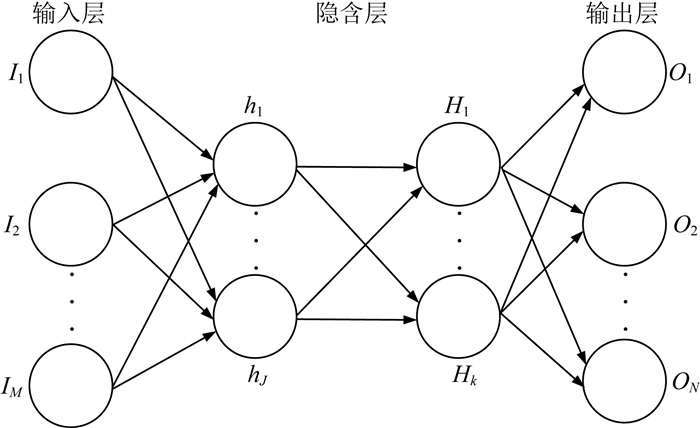
\includegraphics[width=0.7\textwidth]{BP.jpg} % 在命名上面也有要求??? 我靠
            \caption{BP神经网络}
            \label{BP}
    \end{figure}
    BP(Back Propagation)神经网络分为两个过程:(1)、工作信号正向传递子过程 (2)、误差信号反向传递子过程;在BP神经网络中,单个样本有m个输入,有n个输出,在输入层和输出层之间通常还有若干个隐藏层。一个三层的BP网络就可以完成任意的m维到n维的映射。即这三层分别是输入层(I),隐含层(H),输出层(O)。其结构如图\ref{BP}所示。
    \par 在BP神经网络中,输入层和输出层的节点个数都是确定的,而隐含层节点个数不确定,那么应该设置为多少才合适呢?实际上,隐含层节点个数的多少对神经网络的性能是有影响的,有一个经验公式可以确定隐含层    
       节点数目,如下
        \begin{equation} % 等式
            h =\sqrt{m + n} + a \nonumber
        \end{equation}
    其中$h$为隐含层节点数目,$m$为输入层节点数目,$n$为输出层节点数目,$a$为1到10之间的调节常数。
    % \subsection* 取消前面的标号


    \subsection{正向传递子过程}
    % $特殊符号表示$
    现在设节点$i$和节点$j$之间的权值为 $\omega_{ij}$,节点$j$的阈值为$b_{j}$, 每个节点的输出值为$x_{j}$, 而每个节点的输出值是根据上层所有节点的输出值、当前节点与上一层所有节点的权值和当前节点的阀值还有激活函数来实现的.具体计算方法如下
    \begin{equation} % 等式
        % & 右对齐
        \begin{aligned}
        & S_j =\sum\limits_{i=1}^{m-1} \omega_{ij}x_{i} + b_{j} \nonumber \\
        & x_{j}=f(S_{j})
        \end{aligned}
    \end{equation}
    其中, $f$为激活函数, 一般选取$s$型函数或者线性函数。
    正向传递的过程比较简单,按照上述公式计算即可。(在BP神经网络中,输入层节点没有阈值)
    \subsection*{1.2 反向传递子过程}
    在BP神经网络中,误差信号反向传递子过程比较复杂,它是基于Widrow-Hoff学习规则的。假设输出层的所有结果为$d_{j}$,误差函数如下
    \begin{equation} % 等式
        % & 右对齐
        \begin{aligned}
        & E(\omega, b) =\frac{1}{2}\sum\limits_{j=0}^{n-1}(d_{j} - y_{j}) ^ 2 \nonumber 
        \end{aligned}
    \end{equation}
    而BP神经网络的主要目的是反复修正权值和阀值,使得误差函数值达到最小。

    
    \section{BP神经网络PID控制器}
    \begin{figure}[H]
        \centering % 图片居中
        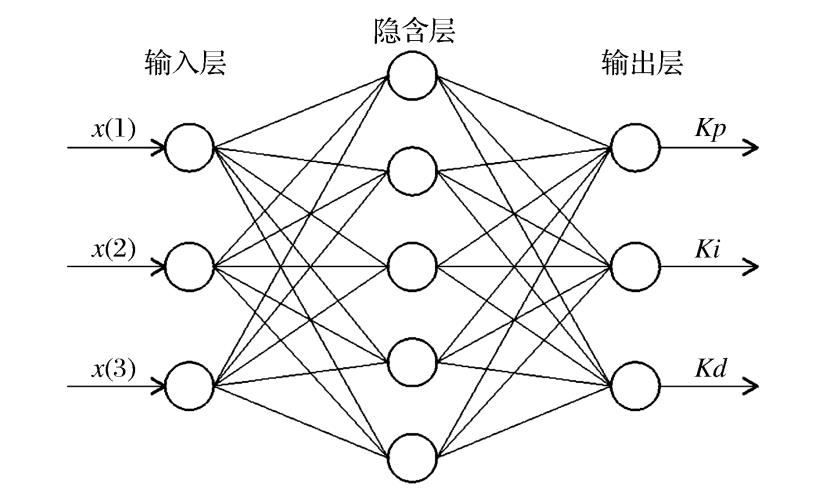
\includegraphics[width=0.7\textwidth]{PID_mode.jpg} % 在命名上面也有要求??? 我靠
        \caption{PID控制神经网络}
        \label{PID_BP}
    \end{figure}
    \subsection{改进型BP神经网络}
    BP神经网络具有多层结构,包括输入层、隐含层和输出层,其中隐含层也可以是多层,具体与实际系统的训练程度相关,而且每一层都可以具有多个节点,也可以包含多个输入和输出值。在PID控制器的设计中,遇到的实际系统一般都是非线性的,采用BP神经网络算法可以通过梯度下降法来利用梯度搜索的技术使得
    神经网络的实际输出值和我们期望的输出值的误差均方差降为最小。
    \par 传统的BP神经网络在训练的时候,大都采用梯度下降法来求解权值和阈值,这种算法是先初始化一个解,然后在此基础上确定搜索方向和步长,这样初始解就会根据这个搜索方向和步长进行移动,从而使得待求解的目标函数输出下降,然后不断迭代下去,使得最后的误差比较小,在此过程中步长的选取显得尤为重要,
    因为搜索算法确定之后整个求解过程都是基于此进行计算的,其运行过程是固定不变的,然而步长不一样,如果步长设置的过大,会使得搜索不仔细,可能引起系统的剧烈震荡,但是设置过小又会导致收敛速度太慢,从而达不到无人机控制系统快速性的要求,所以
    步长的选定就会显得很重要了。学习率$/eta$就是用来对原步长进行调整的,但在传统的BP神经网络算法里它又是固定不变的,而研究将采取自适应改变学习率的方法,对其进行合理的调节,就是在训练误差比较大时,适当减小学习率,在训练误差比较小时,适当增加学习率,以期达到对传统BP神经网络算法来优化的目的。
    根据整个系统的实时运行状态来不断调整权值系数, 不断学习, 使得输出层神经元的输出状态对应于 PID 控制器的 3 个参数 $K_{p}$ 、 $K_{i}$ 、 $K_{d}$ , 使其处于
    实时变化中, 以此达到参数的在线整定 \upcite{6} 。当然这个变化是根据系统的运行状态而变,是一个动态调节的过程,而且最终的网络输出值也是在我们给定的某种最优化控制律下的参数,这样就实现了我们需要对整个无人机系统的自适应控制。
    \par 采用3-5-3的神经网络结构,即输入层、隐含层、输出层分别含3个、5个、3个神经元的三层机构,如图\ref{PID_BP}所示。

    \subsection{BP神经网络PID控制器算法}
    BP神经网络输入神经元$M$ = 4;隐含层神经元$I$ = 5;输出神经元$J$ = 3,第m个输入神经元、第i个隐含层神经元、第j个输出神经元分别用$x_{m}$, $k_{i}$, $y_{j}$表示,$x_{m}$和$k_{i}$之间的权值为$\omega_{mi}$, $k_{i}$和$y_{j}$之间的权值$\omega_{ij}$。BP神经网络层采用正负对称的Sigmoid激活函数。由于网络输出$K_{p}$,$K_{i}$和$K_{D}$为负值,因此
    输出层采用非负的Sigmoid激活函数\upcite{5},神经网络模型如图\ref{PID_BP}所示。\par
    网络输入层的输入、输出为
    \begin{equation} % 等式
        % & 右对齐
        \begin{aligned}
        O_{m}^{(1)} =x_{m}(m=1,2,3,4)  
        \end{aligned}
    \end{equation}
    \par 其中,$x_{1}$ = $r_{m}(k)$为系统的期望输入,$x_{2}$ = $y(k)$为系统的实际输入,$x_{3}$=$e(k)$,$x_{4}$=1为非线性调节的外部偏置常量。
    网络隐含层的输入、输出为
    % 分段函数
    \begin{equation}
        \begin{cases}
        & net_{i}^{(2)}(k)=\sum\limits_{m=1}^{4}\omega_{mi}^{(3)}x_{m}\\
        & O_{i}^{(2)}(k)=f(net_{i}^{(2)}(k)) \hspace{1em}(i=1,2,3,4,5)
        \end{cases}
    \end{equation}

    网络输出层输入、输出为
    \begin{equation}
        \begin{cases}
        & net_{j}^{(3)}(k)=\sum\limits_{i=1}^{5}\omega_{ij}^{(3)}(k)O_{j}^{(2)}(k)\\
        & O_{j}^{(3)}(k)=g(net_{j}^{(3)}(k)) \hspace{1em}(j=1,2,3) \\
        & O_{i}^{(3)}(k)=K_{P}, O_{2}^{(3)}(k)=K_{I}, O_{3}^{(3)}(k)=K_{D} g(net_{j}^{(3)}(k)) \hspace{1em}(j=1,2,3)
        \end{cases}
    \end{equation}
    式中,$\omega_{mi}^{(2)}$、$\omega_{ij}^{(3)}$分别表示隐含层、输出层权值系数,上角标(1)、(2)、(3)分别表示输入层、隐含层、输出层。误差函数的选择根据梯度下降法的思想进行表达,取的性能指标函数为:
    \begin{equation} % 等式
        % & 右对齐
        \begin{aligned}
        E(k) =(r_{m}(k) - y(k))^2/2  
        \end{aligned}
    \end{equation}
    以$\eta$为学习速率,$\alpha$为惯性系数的$\Delta\omega_{ij}^{(3)}$为:
    \begin{equation}
        \begin{cases}
            % \partial导数符号
            % 点乘:a \cdot b
            % 叉乘:a \times b
            % 除以:a \div b
        & \Delta\omega_{ij}^{(3)}(k)=\eta\frac{\partial E(k)}{\partial \omega_{ij}^{(3)}(k)} + \alpha\Delta\omega_{ij}^{(3)}(k-1)  \sum\limits_{i=1}^{5}\omega_{ij}^{(3)}(k)O_{j}^{(2)}(k-1)\\
        & \frac{\partial E(k)}{\partial \omega_{ij}^{(3)}(k)} = \frac{\partial E(K)}{\partial y(k)} \cdot{\frac{\partial y(K)}{\partial u(k)}} \cdot{\frac{\partial u(K)}{\partial O_j^{(3)}(k)}} \cdot{\frac{\partial O_j^{(3)}(k)}{\partial net_{j}^{(3)}(k)}} \cdot{\frac{\partial net_{j}^{(3)}(k)}{\partial \omega_{ij}^{(3)(k)}}}
        \end{cases}
        \label{con:formula1}
    \end{equation}
    用sgn($\frac{\partial y(k)}{\partial u(k)}$)代替$\frac{\partial y(k)}{\partial u(k)}$。由此带来的误差由学习速率$\eta$进行补偿:
    \begin{equation}
        \begin{cases}
            % \partial导数符号
            % 点乘:a \cdot b
            % 叉乘:a \times b
            % 除以:a \div b
        & \frac{\partial net_{j}^{(3)(k)}}{\partial \omega_{ij}^{(3)(k)}} = O_{i}^{(2)}{k}, \frac{\partial u(k)}{\partial O_{i}^{(3)}(k)} = e(k) - e(k-1) = x_{1} \\
        & \frac{\partial u(k)}{\partial O_{2}^{(3)}(k)} = e(k) = x_{2}, \frac{\partial u(k)}{\partial O_{3}^{(3)}(k)} = e(k) - 2e(k-1) = e(k-2) = x_{3}
        \end{cases}
    \end{equation}
    式(\ref{con:formula1})可以写成:
    \begin{equation}
        \begin{cases}
        & \Delta\omega_{ij}^{(3)}(k)=\alpha\Delta\omega_{ij}^{(3)}(k-1) + \eta\delta_{j}^{(3)}O_{j}^{(2)}(k) \\
        & \delta_{j}^{(3)} = -\frac{\partial E(k)}{\partial net_{j}^{(3)}(k)} = e(k) \cdot{sgn(\frac{\partial y(k)}{\partial u(k)})} \cdot{\frac{\partial u(k)}{\partial O_{j}^{(3)}(k)}} \cdot{g'(net_{j}^{(3)}(k))}
        \end{cases}
    \end{equation}
    同理:
    \begin{equation}
        \begin{cases}
        & \Delta\omega_{mi}^{(2)}(k)=\alpha\Delta\omega_{mi}^{(2)}(k-1) + \eta\delta_{i}^{(2)}O_{m}^{(1)}(k) \\
        & \delta_{i}^{(2)} = -\frac{\partial E(k)}{\partial net_{i}^{(2)}(k)} =f'(net_{i}^{(2)}) \cdot{\sum\limits_{j=1}^{3}\omega_{ij}^{(3)}(k)} \cdot{\delta_{j}^{(3)}}             e(k) \cdot{sgn(\frac{\partial y(k)}{\partial u(k)})} \cdot{\frac{\partial u(k)}{\partial O_{j}^{(3)}(k)}} \cdot{g'(net_{j}^{(3)}(k))}
        \end{cases}
    \end{equation}
    \par 其中,$f(x)$=$e^{x}$-$e^{-x}$ / $e^{x}$ + $e^{-x}$, $g(x)$=$e^{x}$ / $e^{x}$ + $e^{-x}$。求导得$f'(x)$=(1-$f^{2}(x)$), $g'(x)$=2$g(x)$(1-$g(x)$)。
    \clearpage % 分页
    \section{结 论}
    实验结果表明:BP神经网络阶跃响应速度较快,根据采样时间判断训练步数克制,BP神经网络在第39步时响应值为1.且无明显超调。传统的PID控制器也无明显超调,响应值在65步时才为1,由此可以证明,BP神经网络PID控制器比传统PID控制器响应快,实际应用中传统PID控制器要比此处的性能要差。
    采用了两种PID控制方法:传统PID控制和BP神经网络PID控制.BP神经网络PID控制效果要明显
优于传统PID控制.传统PID控制器在不采用BP神经网络PID控制器训练过后的比例系数KP、微分系数
KI、积分系数KD的情况下阶跃响应会产生较大幅度的超调和振荡,系统需要更长的时间才能稳定.传统
PID控制器在采用BP神经网络PID控制器训练过后的比例系数KP、微分系数KI、积分系数KD的情况下阶
跃响应超调幅度降低,不会产生超调.BP神经网络PID控制阶跃响应迅速,且不会产生超调和振荡.改进
算法中的BP神经网络PID控制可以避免在快速响应的过程中产生超调和振荡,使系统更加稳定.
    \clearpage % 分页
    
 
    % \clearpage % 分页
    % \section*{以下为一些工具}
    %     \begin{align} % 对齐
    %         & ABCDEFGHIJKLMNOPQRSTUVWXYZ \label{alphabet} \\
    %         & abcdefghijklmnopqrstuvwxyz \\
    %         & \alpha \beta \gamma \delta \epsilon \varepsilon \zeta \eta \theta \lambda \mu \nu \xi \pi \rho \sigma \tau \upsilon \phi \varphi \chi \psi \omega  
    %     \end{align}

    %     \begin{align}
    %         % 不能使用 \[\] 标号来分割开下面三个
    %         \begin{bmatrix}
    %             1 & 2 \\
    %             3 & 4 \\
    %         \end{bmatrix}
    %         \\
    %         \begin{pmatrix}
    %             1 & 2 \\
    %             3 & 4 \\
    %         \end{pmatrix}
    %         \\
    %         \begin{matrix}
    %             1 & 2 \\
    %             3 & 4 \\
    %         \end{matrix}
    %     \end{align}
    
    %     \begin{equation} % 等式
    %     A_{t+1} = \arg\min_A \ \mathcal{L}(A,E_t,\Delta\tau_t,W_t,b_t), \nonumber
    %     \end{equation}
    
    %     \begin{equation}
    %         \begin{aligned} \label{eq:rasl}
    %             \min_{A,E,\Delta \tau} \quad & \sum_{i=1}^{N}||A_i||_* + \lambda ||E_i||_1  \\
    %             \mathrm{s.t.} \quad & D_i \circ \tau_i + \sum_{k=1}^{n_i} J_{ik} \Delta \tau_i \epsilon_k \epsilon_k^T = A_i + E_i, \\
    %             & i = 1,2,\cdots,N. 
    %         \end{aligned}
    %     \end{equation}
    
    %     % 标准表格的形式
    %     \begin{table}[htbp]
    %         \centering  % 显示位置为中间
    %         \caption{standard table}  % 表格标题
    %         \label{table1}  % 用于索引表格的标签
    %         %字母的个数对应列数,|代表分割线
    %         % l代表左对齐,c代表居中,r代表右对齐
    %         \begin{tabular}{|c|c|c|c|}  
    %             \hline  % 表格的横线
    %             & & & \\[-6pt]  %可以避免文字偏上来调整文字与上边界的距离
    %             1&2&3&4 \\  % 表格中的内容,用&分开,\\表示下一行
    %             \hline
    %             & & & \\[-6pt]  %可以避免文字偏上 
    %             0.1&0.2&0.3&0.4 \\
    %             \hline
    %         \end{tabular}
    %     \end{table}        

    %     \begin{table}[htbp]
    %         \caption{Title of table} \label{tab:table}
    %         \centering
    %         \addtolength{\tabcolsep}{-0mm} % 控制列间距
    %         \begin{tabular}{ccccc}
    %             \toprule[0.75pt]	% package booktabs
    %             \multicolumn{4}{c}{table head} \\
    %             \midrule[0.5pt]	% package booktabs
    %             \multirow{4}{*}{text} & 1 & 2 & 3 & 4 \\  % package multirow
    %             & 5 & 6 & 7 & 8 \\
    %             \cmidrule[0.5pt]{2-4}	% package booktabs
    %             & 9 & 10 & 11 & 12 \\
    %             & 13 & 14 & 15 & 16 \\
    %             \bottomrule[0.75pt]	% package booktabs
    %         \end{tabular}
    %     \end{table}

    %     % \eqref{eq:alphabet} : eq:alphabet eq 代表的是公式
    %     % \begin{figure}
    %     %     \centering % 图片居中
    %     %         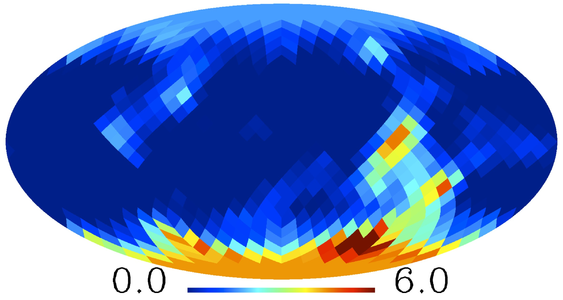
\includegraphics[width=\textwidth]{figure1.jpg}
    %     %     \caption{摩擦角}
    %     %     \label{fraction}
    %     % \end{figure}
    %     引用: Eq. \eqref{alphabet}, Fig. \ref{figure:fraction},  \\
    %     \clearpage % 分页
        
    % \end{multicols}
        % 引用图片的时候, 要想引用成功, 必须要把标签加在图片命名之后:
    
        % \begin{algorithm}
        %     \caption{Title of the Algorithm}
        %     \label{algo:ref}
        %     \begin{algorithmic}[1]
        %         \REQUIRE some words.  % this command shows "Input"
        %         \ENSURE ~\\           % this command shows "Initialized"
        %         some text goes here ... \\
        %         % \WHILE {条件} 
        %         \WHILE {\emph{not converged}}
        %         \STATE ... \\  % line number at left side
        %         \ENDWHILE
        %         \RETURN this is the lat part.  % this command shows "Output"
        %     \end{algorithmic}
        % \end{algorithm}
        % \clearpage % 分页
        % plain,按字母的顺序排列,比较次序为作者、年度和标题.
        % unsrt,样式同plain,只是按照引用的先后排序.
        % alpha,用作者名首字母+年份后两位作标号,以字母顺序排序.
        % abbrv,类似plain,将月份全拼改为缩写,更显紧凑.
        % ieeetr,国际电气电子工程师协会期刊样式.
        % acm,美国计算机学会期刊样式.
        % siam,美国工业和应用数学学会期刊样式.
        % apalike,美国心理学学会期刊样式.
        % http://blog.sina.com.cn/s/blog_6fda97ea0102ycjp.html
    % 文献引用
    % \bibliographystyle{plain}

\addcontentsline{toc}{section}{参考文献}
\renewcommand{\refname}{参考文献}   % 将References改为参考文献
% \cite{author1.year1,author2.year2}  “99” 表示以最多两位数来编号参考文献, 用于对齐
\begin{thebibliography}{99}
\addtolength{\itemsep}{-2ex} % 用于更改行距
\bibitem{1}张岳平,朱力超,孙涛.用Hopfield神经网络与模拟退火算法求解UAV航路规划问题[J].海军航空工程学院学报,2007,22(4):451-453,466. DOI:10.3969/j.issn.1673-1522.2007.04.012.
\bibitem{2}陈侠,艾宇迪.应用改进神经网络的无人机三维航迹规划[J].电光与控制,2018,25(9):7-11. DOI:10.3969/j.issn.1671-637X.2018.09.002.
\bibitem{3}缪永飞.多UAV联合搜救任务规划建模及优化方法研究[D].湖北:武汉理工大学,2017.
\bibitem{4}苏续军,吕学志.BP神经网络模型在无人机系统故障预测中的应用分析[J].计算机应用与软件,2019,36(9):70-75. DOI:10.3969/j.issn.1000-386x.2019.09.013.
\bibitem{5}张永振,苏寒松,刘高华,等.基于BP神经网络的PID控制器参数调整[J].南开大学学报(自然科学版),2018,51(3):26-30.
\bibitem{6}高富强,李萍,张磊敏,等.基于BP神经网络整定的PID控制及其仿真[J].山东陶瓷,2017,40(3):27-31. DOI:10.3969/j.issn.1005-0639.2017.03.007.
\bibitem{7}余后明,刘彦臣,郑士振,等.基于改进型BP神经网络的四旋翼控制系统[J].甘肃科学学报,2019,31(2):87-91. DOI:10.16468/j.cnki.issn1004-0366.2019.02.015.
\bibitem{8}虞晓霞.无人机飞行姿态稳定控制技术研究[D].吉林:长春理工大学,2018.
\bibitem{9}朱凯光,王昊,彭聪,张琼,范天姣,景春阳.基于BP神经网络的固定翼航空电磁线圈姿态校正[J].吉林大学学报(地球科学版),2020,50(01):252-260.

\end{thebibliography}  

\end{document}